\documentclass[UTF8]{ctexart}

\usepackage{mathtools,mathabx,bm,lmodern}
\usepackage{booktabs,siunitx,xltxtra}
\usepackage{datetime}
\usepackage[a4paper,hmargin=1.2in,vmargin=1in]{geometry}
\usepackage{graphicx,tikz,wrapfig}
\usepackage{fancyhdr}
\usepackage{subfigure}
\usepackage{float}
\usepackage{footnote}
\usepackage{listings}
\usepackage{array,tabularx}
\usepackage{verbatim}%多行注释
\usepackage{ragged2e} 
\usepackage{booktabs,makecell, multirow, tabularx}
\usepackage{caption}
\usepackage{multicol}
%\usepackage{bibtex}
\usepackage[utf8]{inputenc}

\usepackage{tikz,mathpazo,xcolor}
\usetikzlibrary{arrows.meta}%箭头
\usepackage{mhchem,chemfig,extarrows}  %化学式
\usepackage{geometry}
\geometry{a4paper,centering,scale=0.9}

\title{变温霍尔效应实验报告}
\author{PB22020469 文义钧}

\begin{document}
\maketitle

\section{实验原理}
使用范德堡法测量电阻率: 找4个电极A,B,C,D.在A,B接入电流$I_{AB}$, 测量C,D电压$V_{CD}$, 并通$I_{BC}$, 测$V_{DA}$:
$R_{AB,CD}=\dfrac{|V_{CD}|}{I_{AB}},\;R_{BC,DA}=\dfrac{|V_{DA}|}{I_{BC}}$, 
实验中为减少电流引起的误差每个点测两个电流方向的电压$V_{M1}, V_{M2}$并求平均值, 并可求得电阻率(范德堡因子取1)$$\rho=\dfrac{\pi d}{4I\ln 2}(|V_{M1}|+|V_{M2}|+|V_{N1}|+|V_{N2}|)$$\par
在垂直于样品表面处加上磁场$B$, 即可测的霍尔电极电压和不加磁场时的电压差$V_{H}$. 为减少霍尔效应的负效应, 使用不同的B和I使用异号测量法测量四组电势差并轮加$\overline{V_H}=\frac14(V_{H1}-V_{H2}+V_{H3}-V_{H4})$
由于$$R_{H}=\dfrac{d \overline{V_{H}}}{BI}=\dfrac1{nq},\quad\sigma=\dfrac1\rho=nq\mu$$, 故可得霍尔迁移率$$\mu_{H}=R_{H}\sigma$$.
\section{实验仪器}
变温霍尔效应仪、可换向永磁磁铁、SV-12 变温恒温器、TCK-100控温仪、
CVM-2000 电输运性质测试仪、连接电缆和装在恒温器内的霍尔探头、碲镉汞单晶、液氮。
\section{实验过程}
\begin{enumerate}
    \item 打开控温仪和电输运性质测试仪的电源;
    \item 调节变温霍尔效应仪中磁铁角度至测试仪显示电压的极大值, 并作标记;
    \item 测量室温下样品的不同磁场方向、电流方向的霍尔电压和无磁场下不同电流方向的霍尔电压;
    \item 向变温霍尔效应仪中添加液氮, 并等待控温仪显示温度达到80K;
    \item 使用控温仪加热, 重复第三步记录$80\sim300$的至少20个节点;
    \item 计算其
    \item 将记录的数据进行分析, 绘制图表曲线.
\end{enumerate}
\section{实验结果}
已知$$
d=1.1{\rm mm},\;\;B=0.55{\rm T},\;\;I= 5{\rm mA}$$,
原始数据及计算得到结果如下:\\
\begin{table}[!ht]
    \centering
    \begin{tabular}{|l|l|l|l|l|l|l|l|l|}
    \hline
        $T(K)$ &$V_{H1}$(mV) & $V_{H2}$(mV) &$V_{H3}$(mV) & $V_{H4}$(mV) & $V_{M1}$(mV) & $V_{M2}$(mV) & $V_{N1}$(mV) & $V_{N2}$(mV) \\ \hline
        88 & 9.667 & -10.373 & 12.344 & -13.014 & 16.265 & -15.799 & 14.787 & -15.066 \\ \hline
        99 & 9.729 & -10.355 & 13.127 & -13.77 & 17.92 & -17.34 & 16.22 & -16.43 \\ \hline
        108 & 9.528 & -10.1 & 13.154 & -13.79 & 19.75 & -19.17 & 17.83 & -18.01 \\ \hline
        114 & 9.506 & -10.144 & 13.372 & -14.022 & 20.45 & -19.97 & 18.63 & -18.83 \\ \hline
        121 & 9.363 & -9.888 & 12.944 & -13.525 & 21.87 & -21.37 & 19.91 & -20.1 \\ \hline
        128 & 8.96 & -9.43 & 12.585 & -13.103 & 22.83 & -22.39 & 21.02 & -21.23 \\ \hline
        138 & 7.02 & -7.23 & 10.158 & -10.6 & 23.02 & -22.63 & 21.1 & -21.29 \\ \hline
        155 & -15.29 & 15.8 & -16.15 & 16.2 & 25.29 & -15.28 & 14.2 & -14.36 \\ \hline
        165 & -43.8 & 43.8 & -45.5 & 44.8 & 8.57 & -8.67 & 7.8 & -7.87 \\ \hline
        175 & -51.67 & 51.5 & -53.2 & 52.8 & 4.77 & -4.81 & 4.34 & -4.35 \\ \hline
        185 & -35.53 & 35.45 & -35.63 & 35.44 & 2.3 & -2.35 & 2.03 & -2.03 \\ \hline
        195 & -20.57 & 20.66 & -20.6 & 20.66 & 1.28 & -1.33 & 1.12 & -1.11 \\ \hline
        205 & -12.81 & 12.85 & -12.56 & 12.61 & 0.778 & -0.81 & 0.672 & -0.655 \\ \hline
        220 & -6.49 & 6.5 & -6.24 & 6.27 & 0.4 & -0.413 & 0.344 & -0.33 \\ \hline
        230 & -4.18 & 4.22 & -4.09 & 4.15 & 0.267 & -0.287 & 0.24 & -0.216 \\ \hline
        240 & -2.9 & 2.95 & -2.85 & 2.89 & 0.193 & -0.206 & 0.178 & -0.151 \\ \hline
        250 & -2.17 & 2.2 & -2.14 & 2.18 & 0.156 & -0.154 & 0.141 & -0.115 \\ \hline
        260 & -1.72 & 1.75 & -1.64 & 1.68 & 0.13 & -0.12 & 0.115 & -0.095 \\ \hline
        270 & -1.31 & 1.33 & -1.28 & 1.3 & 0.107 & -0.094 & 0.088 & -0.076 \\ \hline
        280 & -1.03 & 1.04 & -0.983 & 0.986 & 0.09 & -0.072 & 0.073 & -0.065 \\ \hline
        301.25 & -0.666 & 0.684 & -0.663 & 0.68 & 0.066 & -0.053 & 0.057 & -0.044 \\ \hline
    \end{tabular}
    表1. 原始数据表
\end{table}\\
\begin{table}[!ht]
    \centering
    \begin{tabular}{|l|l|l|l|l|l|}
    \hline
        $T$(K) & $R_H(\times10^{-3}m^3/C)$& $\rho(\times10^{-3}\Omega m)$ & $\sigma(\times 10^3(\Omega m)^{-1})$ & $\mu_H(m^2\Omega/V)$ & $1/T(K^{-1})$ \\ \hline
        88 & 4.5398 & 15.43466 & 0.06479 & 0.29413 & 0.01136 \\ \hline
        99 & 4.6981 & 16.92859 & 0.05907 & 0.27752 & 0.01010 \\ \hline
        108 & 4.6572 & 18.63616 & 0.05366 & 0.24990 & 0.00926 \\ \hline
        114 & 4.7044 & 19.41391 & 0.05151 & 0.24232 & 0.00877 \\ \hline
        121 & 4.572 & 20.75254 & 0.04819 & 0.22031 & 0.00826 \\ \hline
        128 & 4.4078 & 21.80450 & 0.04586 & 0.20215 & 0.00781 \\ \hline
        138 & 3.5008 & 21.94659 & 0.04557 & 0.15951 & 0.00725 \\ \hline
        155 & -6.344 & 17.23271 & 0.05803 & -0.36814 & 0.00645 \\ \hline
        165 & -17.79 & 8.20380 & 0.12189 & -2.16851 & 0.00606 \\ \hline
        175 & -20.917 & 4.55434 & 0.21957 & -4.59276 & 0.00571 \\ \hline
        185 & -14.205 & 2.17123 & 0.46057 & -6.54238 & 0.00541 \\ \hline
        195 & -8.249 & 1.20651 & 0.82883 & -6.83705 & 0.00513 \\ \hline
        205 & -5.083 & 0.72665 & 1.37618 & -6.99511 & 0.00488 \\ \hline
        220 & -2.55 & 0.37068 & 2.69775 & -6.87927 & 0.00455 \\ \hline
        230 & -1.664 & 0.25177 & 3.97184 & -6.60914 & 0.00435 \\ \hline
        240 & -1.159 & 0.18148 & 5.51038 & -6.38653 & 0.00417 \\ \hline
        250 & -0.869 & 0.14109 & 7.08756 & -6.15909 & 0.00400 \\ \hline
        260 & -0.679 & 0.11467 & 8.72077 & -5.92141 & 0.00385 \\ \hline
        270 & -0.522 & 0.09099 & 10.99057 & -5.73708 & 0.00370 \\ \hline
        280 & -0.4039 & 0.07478 & 13.37185 & -5.40089 & 0.00357 \\ \hline
        301.25 & -0.2693 & 0.05484 & 18.23435 & -4.91051 & 0.00332 \\ \hline
    \end{tabular}\\
    表2. 数据处理表
\end{table}
\begin{minipage}[!ht]{0.8\linewidth}
    \centering
    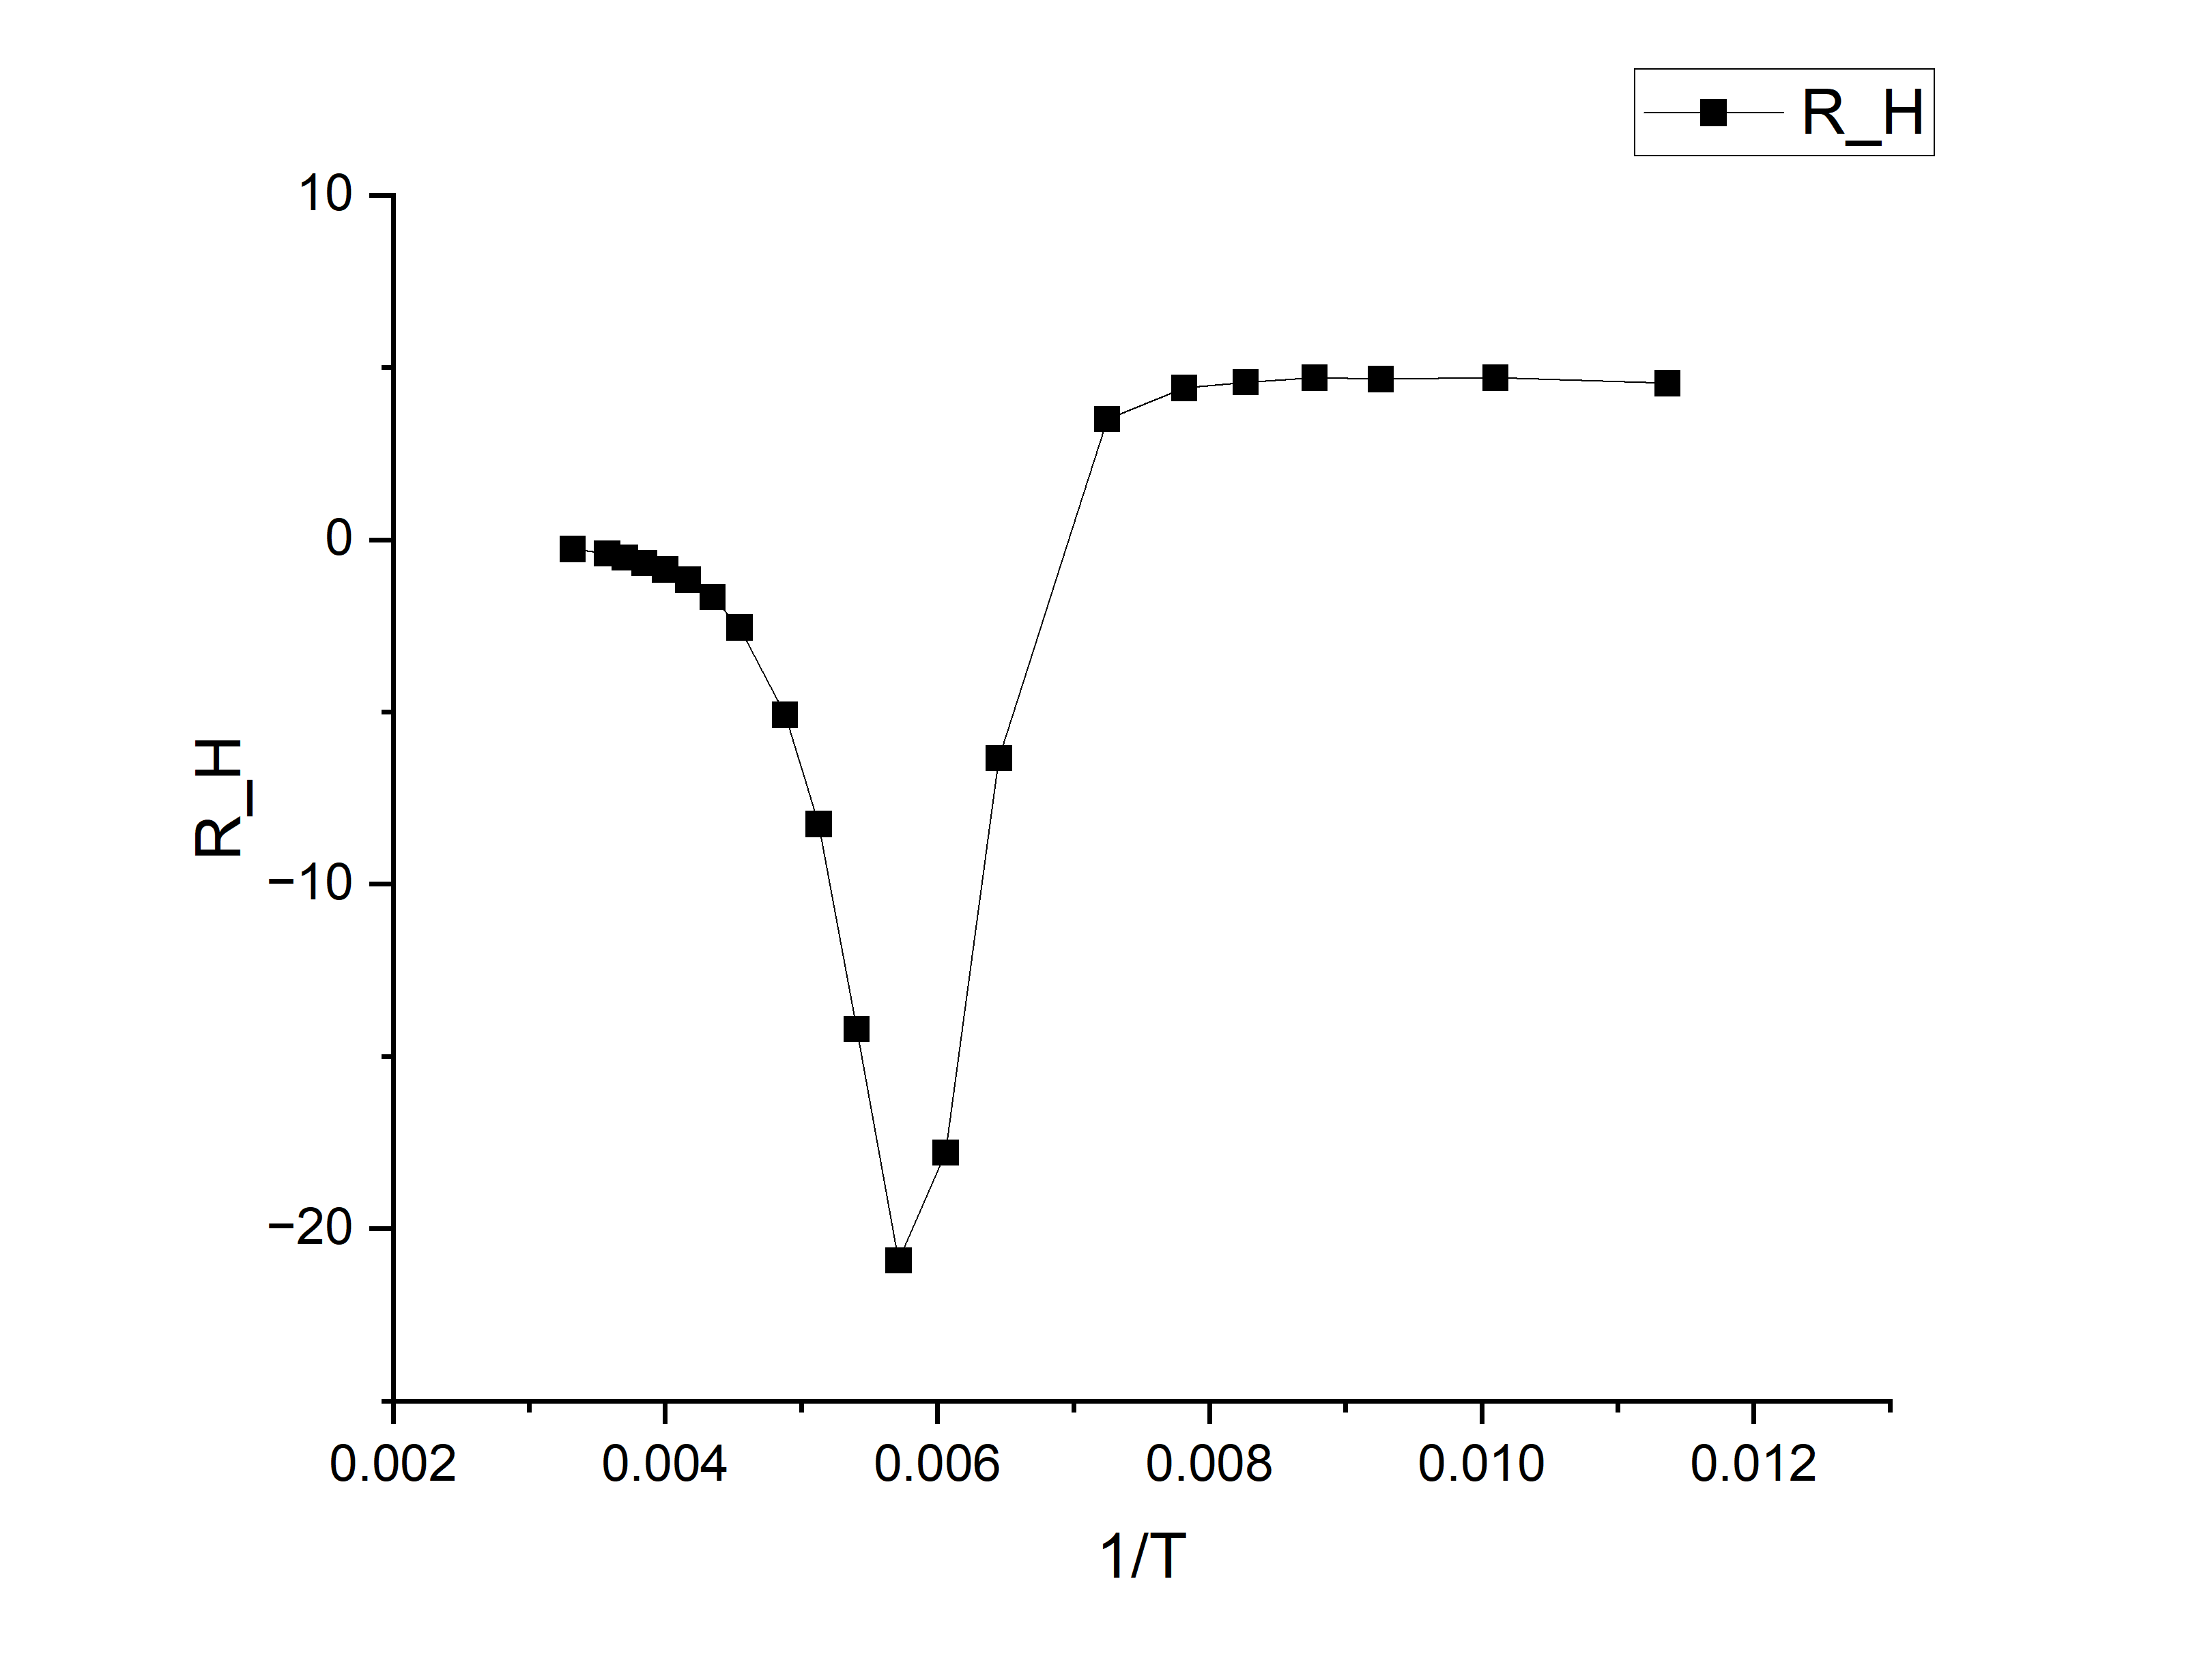
\includegraphics[width=0.9\textwidth]{R.png}\\
    {\small{
        图1. $R_H\sim \frac 1T$曲线
    }}
    \vspace{10pt}
\end{minipage}\\
\begin{minipage}[!ht]{0.8\linewidth}
    \centering
    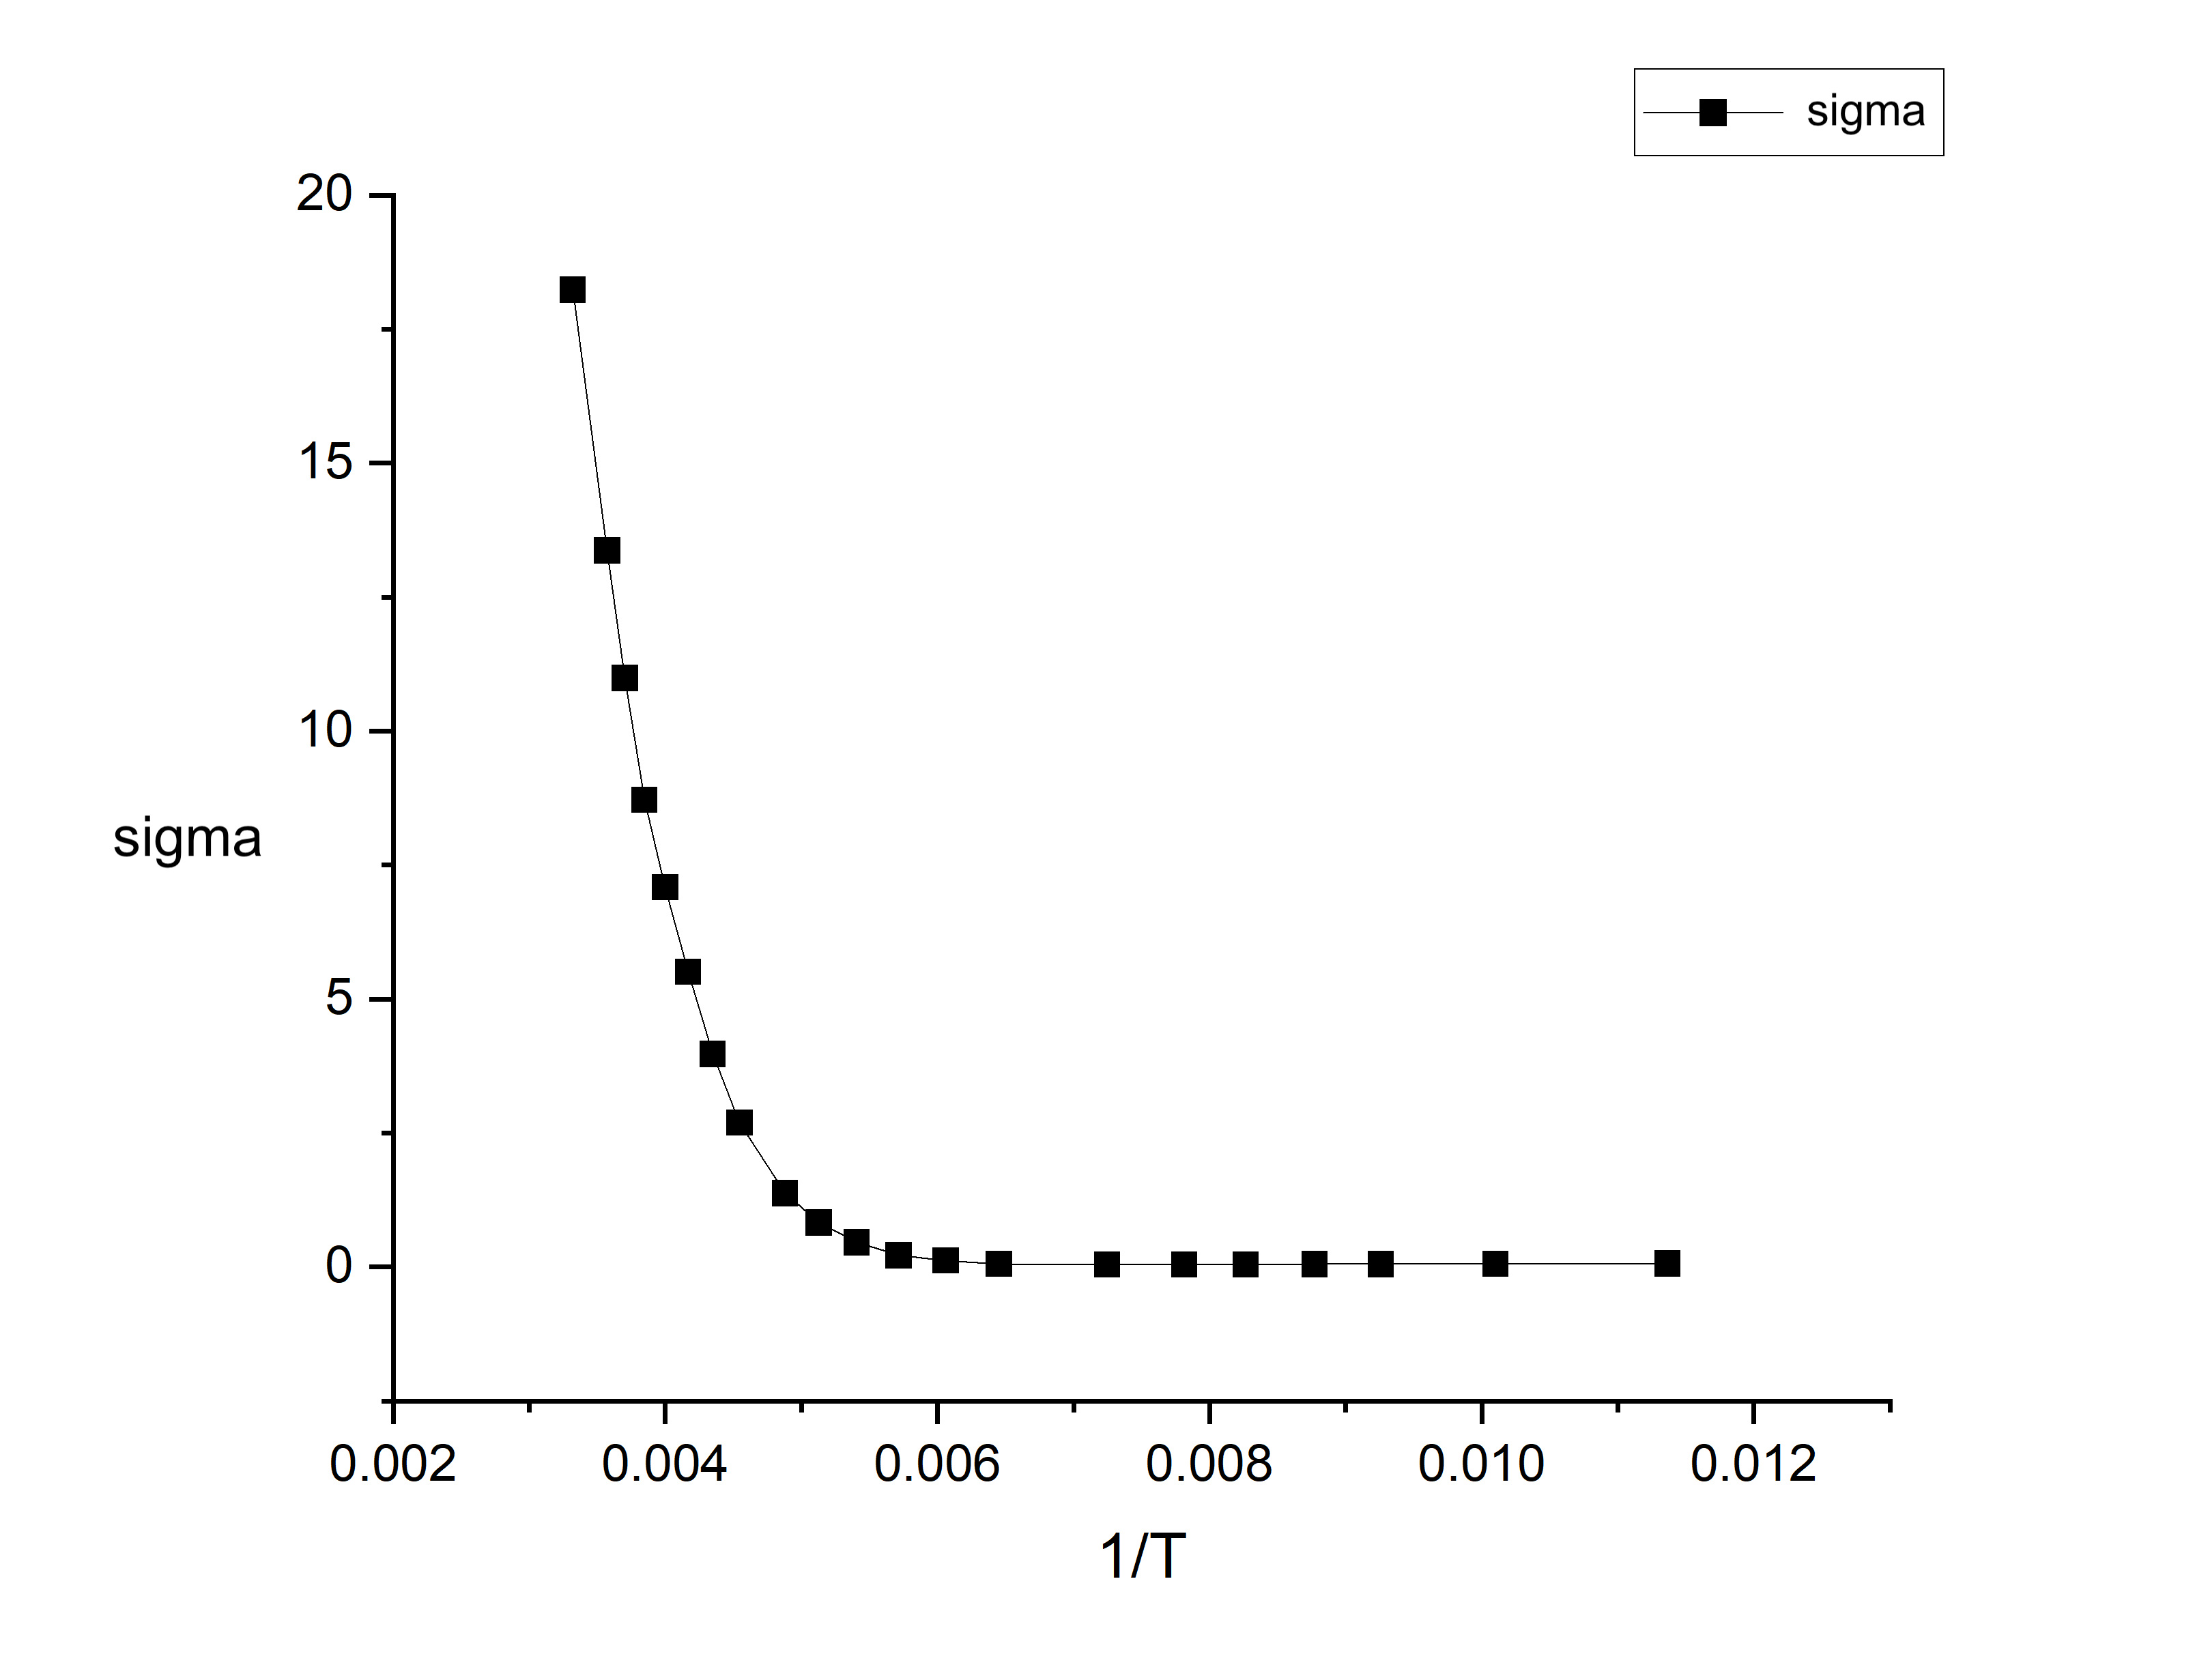
\includegraphics[width=0.9\textwidth]{delta.png}\\
    {\small{
        图2. $\sigma\sim\frac1T$曲线
    }}
    \vspace{10pt}
\end{minipage}\\
\begin{minipage}[!ht]{0.8\linewidth}
    \centering
    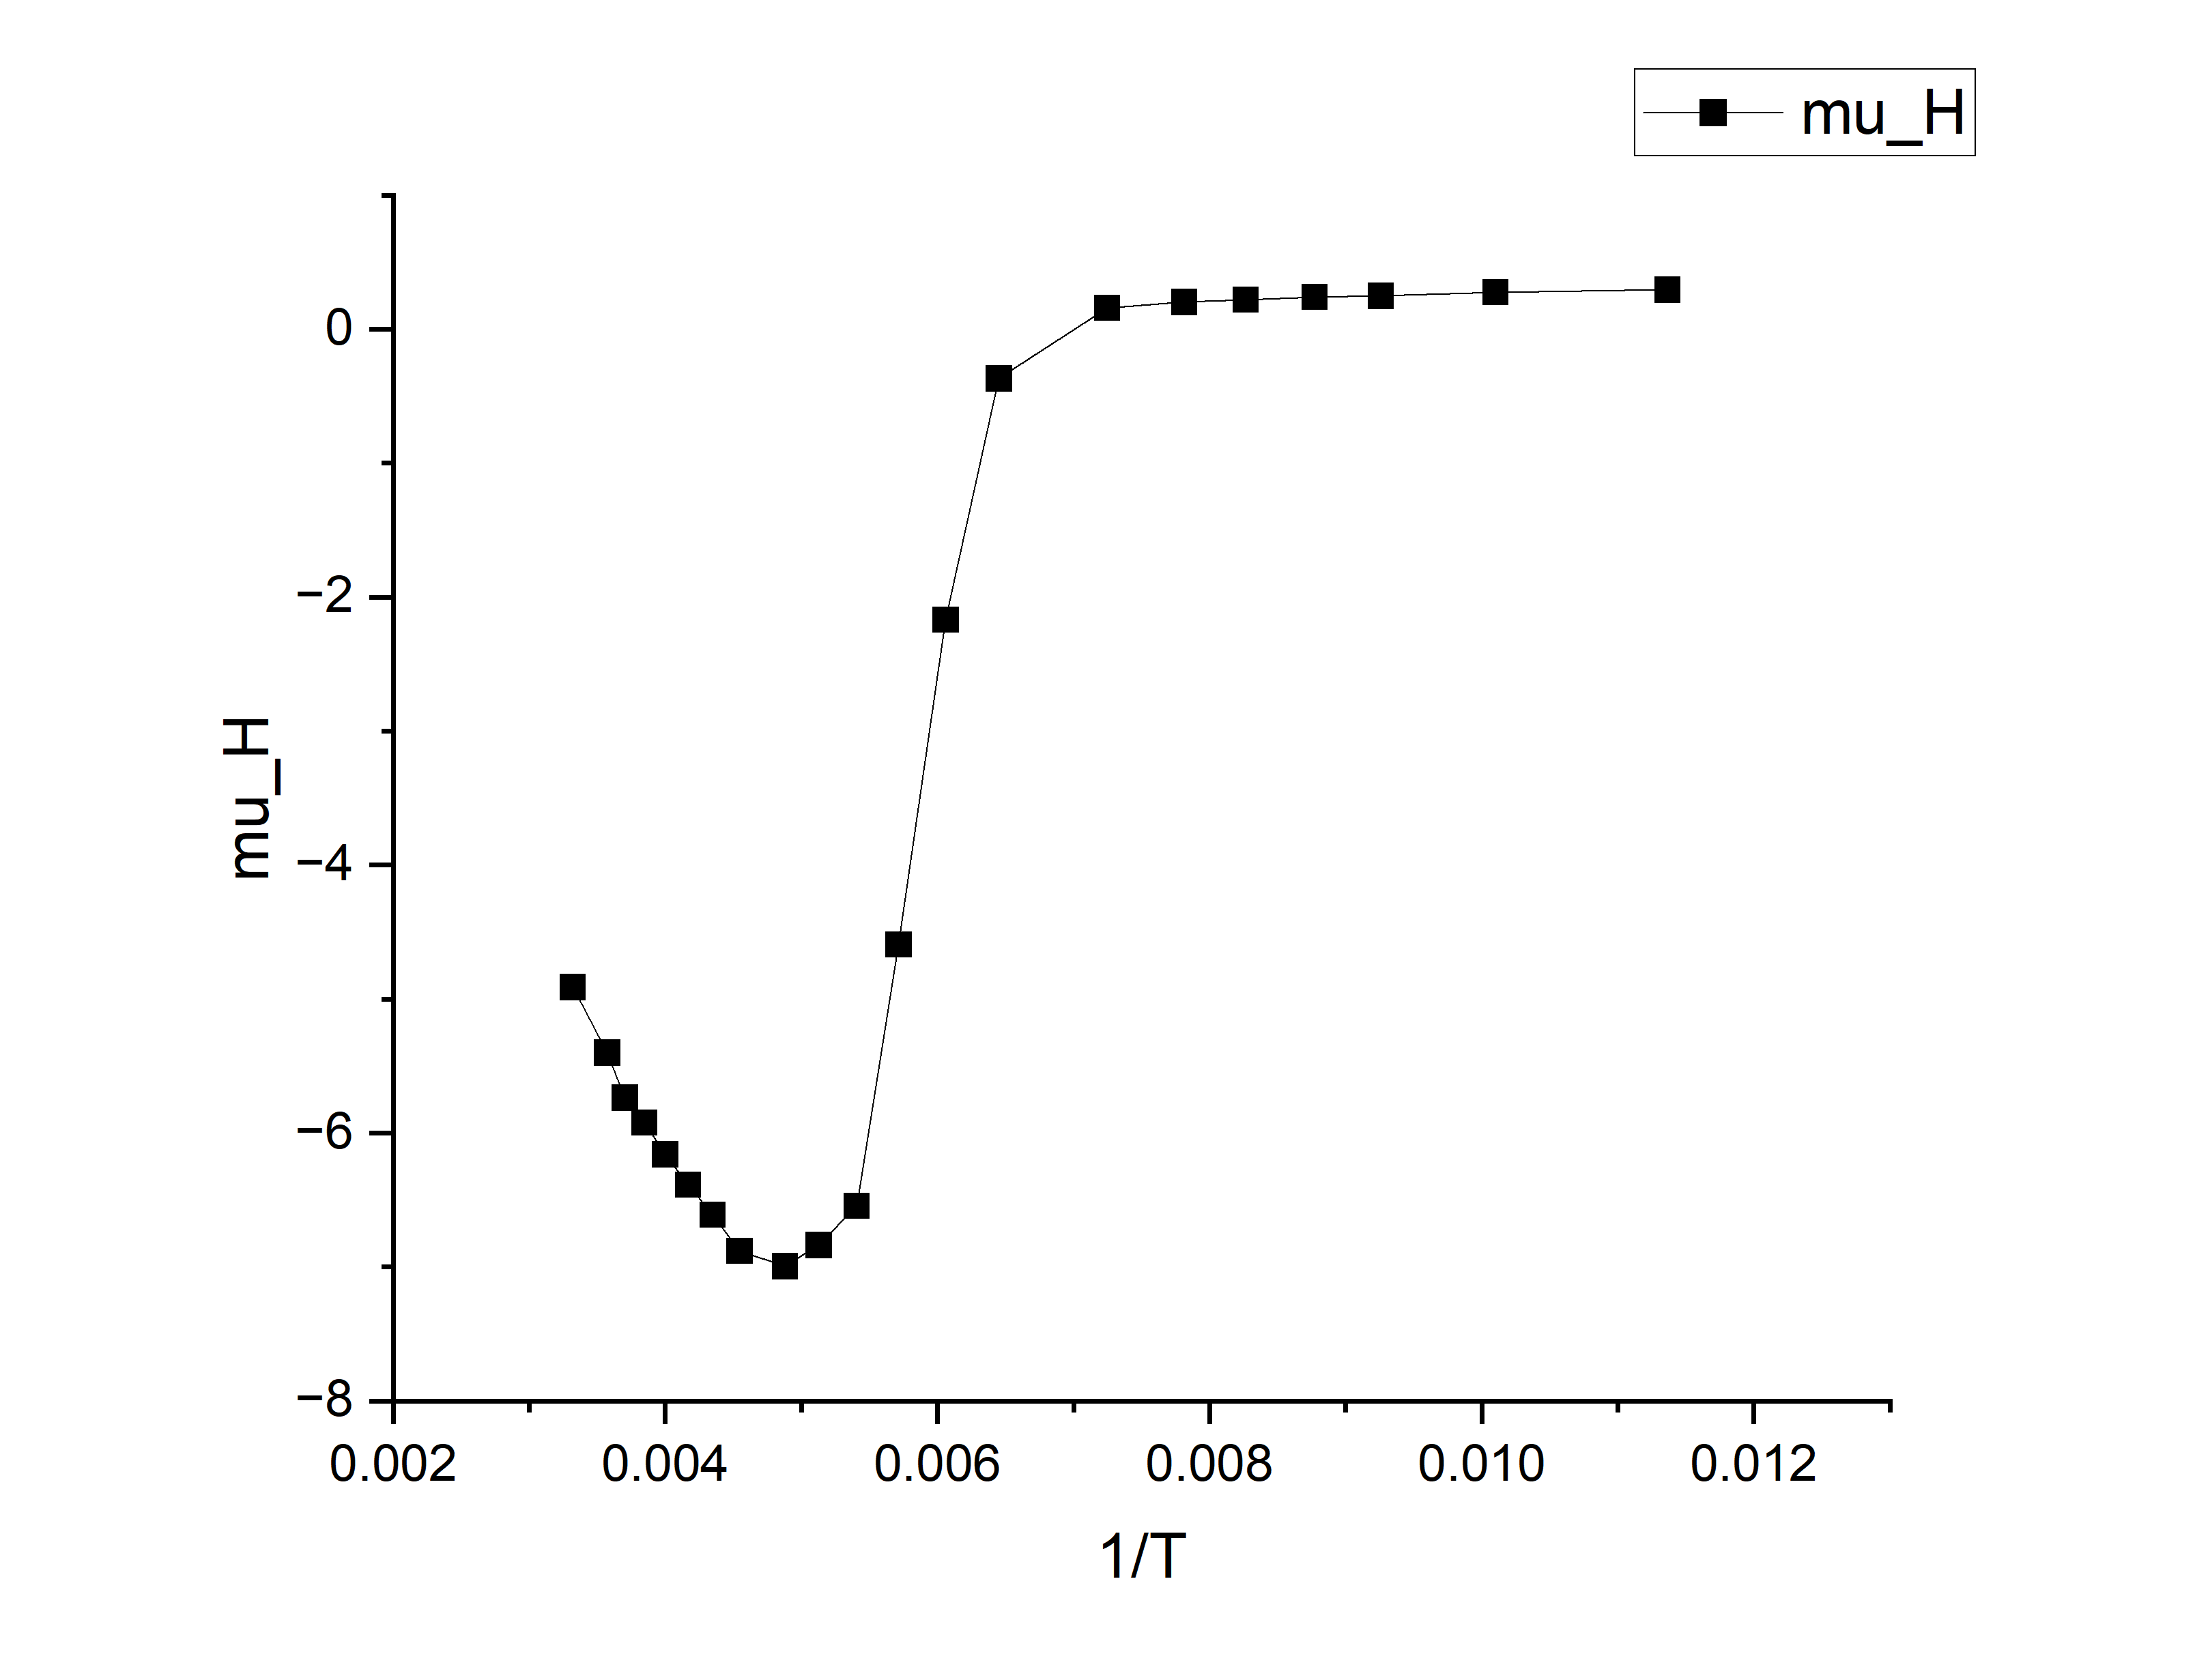
\includegraphics[width=0.9\textwidth]{mu.png}\\
    {\small{
        图3. $\mu_H\sim\frac1T$曲线
    }}
    \vspace{10pt}
\end{minipage}\\
\section{结论}
\begin{enumerate}
    \item 霍尔系数在高温区域(1/T低)时, 霍尔系数的绝对值随温度升高而降低, 说明载流子浓度随温度升高而增大, 属于本征导电.\par 低温区域的霍尔系数比较平坦,说明载流子浓度不随温度显著变化, 说明是掺杂调流
    \item 电导率在高温区域中, 电导率随温度增加, 说明激发了电子和空穴. 低温地区导电率较稳定.
    \item 霍尔迁移率高温时随着温度升高而减小; 在低温时杂质散射为主导, 迁移率变化缓慢.
\end{enumerate}

\subsection{思考题}
\begin{enumerate}
    \item 分别以p型、n型半导体样品为例, 说明如何确定霍尔电场的方向。\par N型半导体的载流子是电子, 电子受洛伦兹力向电势低的一侧具体. p型半导体载流子是空穴
    \item 霍尔系数的定义及其数学表达式是什么?从霍尔系数中可以求出哪些重要参数?\par 霍尔系数是霍尔电场强度与电流密度和外加磁场的积的比 $R_H=\dfrac{E_H}{J\cdot B}=\dfrac1{nq}$.\par 由洛伦兹力与库仑力平衡得$qE_{H}=qvB\Rightarrow E_{H}=vB$, 电流密度$j=nqv$, 故$$R_H=\dfrac{E_H}{J\cdot B}=\dfrac{vB}{nqvB}=\dfrac1{nq}$$ 通过霍尔系数可以得到半导体的载流子类型和材料的载流子浓度
    \item 霍尔系数测量中有哪些副效应,通过什么方式消除它们?\par 载流子本身的速度分布、端点的扩散电流、热扩散电流、材料不均匀对成. 通过测量不同方向磁场电流的值并去平均
    \item 根据霍尔系数与载流子浓度的关系,说明霍尔元件都用半导体材料制成而不用金属材料。 \par 由$R_H=\dfrac 1{nq}$, 金属材料的载流子密度很高, 霍尔系数很小. 半导体载流子密度低, 霍尔系数较大.
    \item 导致实验误差的主要因素有哪些?\par 温度变化, 霍尔系数和电阻率对温度敏感, 在温度调节时温度会在附近波动产生误差.\par 磁场强度均匀性不强, 本次试验全靠手调磁场强度, 可以改进仪器.\par 样品厚度或电阻率可能并不均匀, 导致霍尔电压测量值出现波动.
\end{enumerate}

\begin{minipage}[!ht]{1\linewidth}
    \centering
    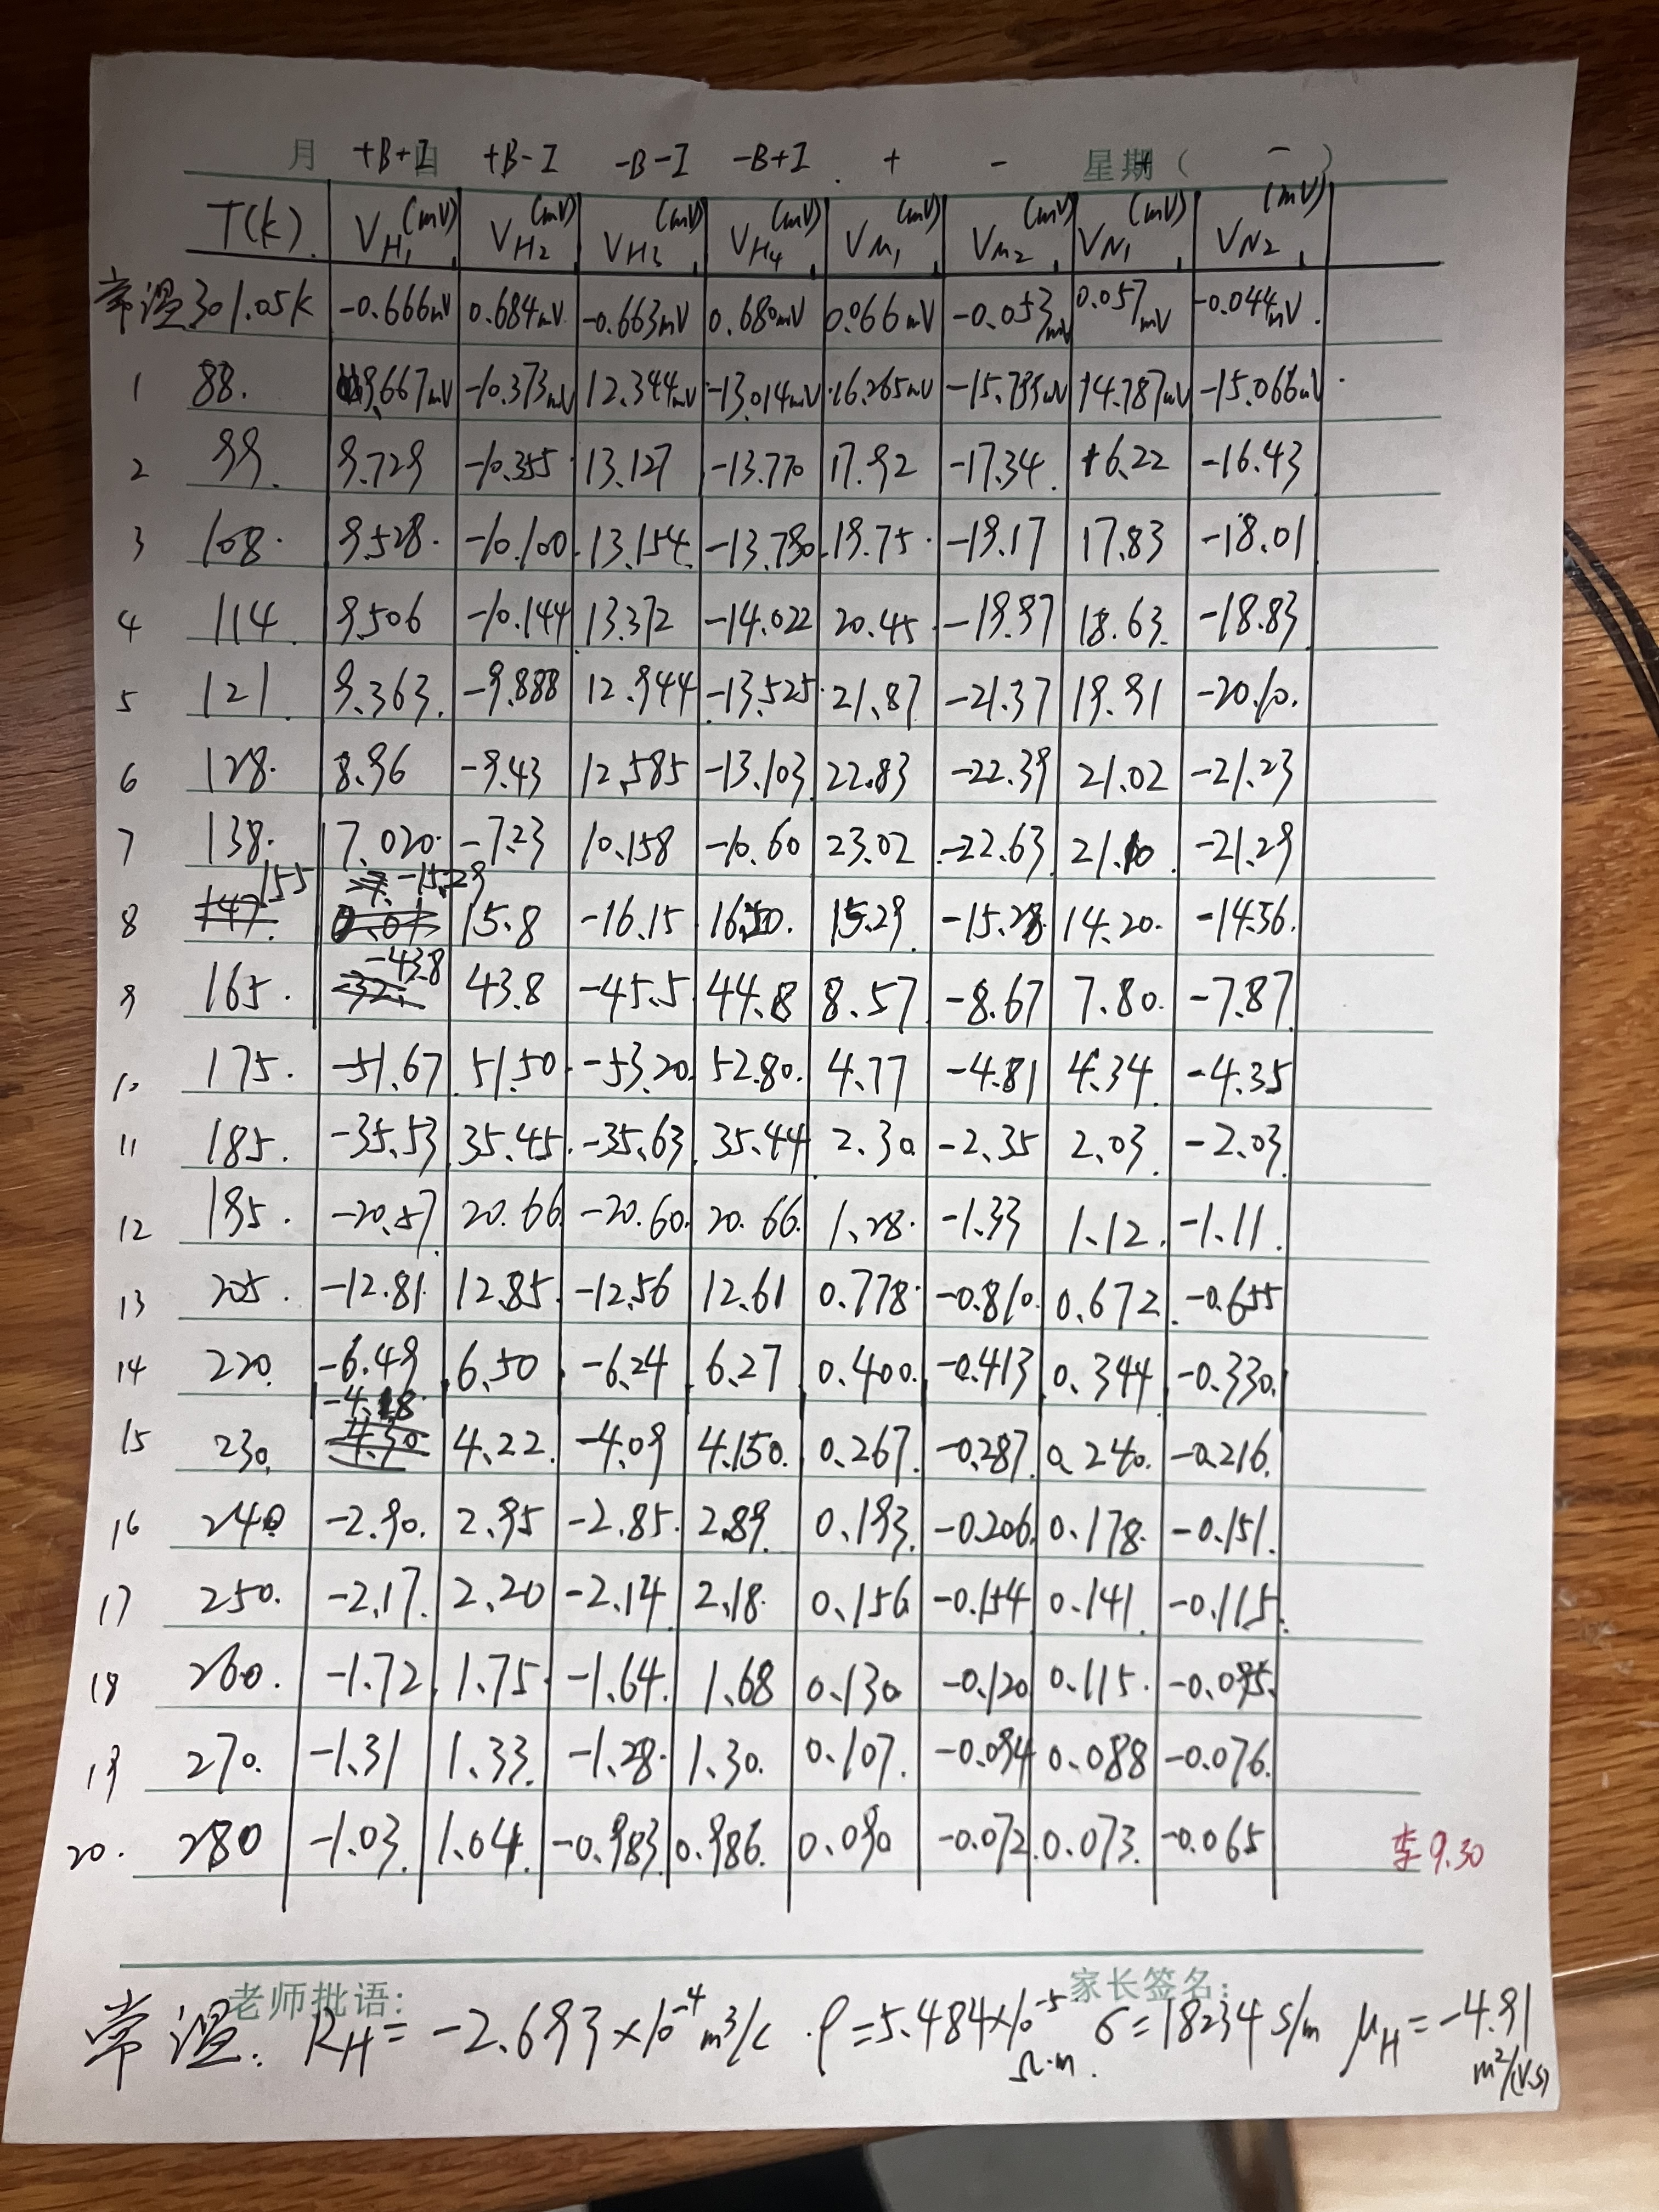
\includegraphics[width=1\textwidth]{photo.jpeg}\\
    {\small{
        图4. 实验原始数据照片
    }}
    \vspace{10pt}
\end{minipage}\\
\end{document}
